\chapter{Results and Discussion}\label{ch:results}
\section{Evidence scope}
Table~\ref{tab:coverage} reports mean Coverage and sample SD for five runs per dataset and configuration, giving $5\times4\times5=100$ reported runs.

\section{Five-run Coverage comparison}
\begin{table}[htbp]
\centering\small
\caption{Coverage mean $\pm$ sample SD (\%) across five datasets and four configurations: three runs per cell ($n=3$; 60 runs in total).}\label{tab:coverage}
\begin{tabular}{lrrrr}
\toprule
Graph & Non-Private & Uniform1 & PDP-PrivIM & Uniform4\\ \midrule
Email & 96.451 $\pm$ 2.100 & 85.417 $\pm$ 1.518 & 90.355 $\pm$ 4.045 & 97.608 $\pm$ 1.541 \\
Bitcoin & 99.070 $\pm$ 0.386 & 82.324 $\pm$ 3.734 & 96.952 $\pm$ 1.734 & 97.387 $\pm$ 0.992 \\
LastFM & 96.270 $\pm$ 1.343 & 80.877 $\pm$ 0.164 & 95.640 $\pm$ 1.058 & 95.088 $\pm$ 0.298 \\
HepPh & 94.945 $\pm$ 0.470 & 83.649 $\pm$ 3.219 & 93.509 $\pm$ 0.000 & 95.788 $\pm$ 0.120 \\
Facebook & 95.238 $\pm$ 3.150 & 82.589 $\pm$ 0.439 & 91.395 $\pm$ 1.843 & 95.650 $\pm$ 2.144 \\
\bottomrule\end{tabular}
\par\vspace{3pt}\begin{minipage}{.97\textwidth}\footnotesize Each cell reports mean Coverage and sample SD for three runs. Five cells report subsets of larger development cohorts; see Appendix~\ref{sec:sourceprotocol} for the selection procedure and full-cohort summaries.\end{minipage}
\end{table}

For the development configurations in Table~\ref{tab:coverage}, PDP-PrivIM has higher mean Coverage than Uniform1 on all five datasets. The differences, computed from the unrounded means, are 4.938 percentage points on Email, 14.628 on Bitcoin, 14.762 on LastFM, 9.860 on HepPh, and 8.806 on Facebook. As the configurations differ in their optimization settings, these gaps describe the combined differences between the evaluated configurations.

Relative to Non-Private, PDP-PrivIM has lower mean Coverage on all five datasets, with gaps ranging from 0.630 percentage points on LastFM to 6.096 on Email. Non-Private provides an unconstrained utility reference, but its training also differs in clipping, slot organization, projection, and sampling. The observed gaps therefore cannot be assigned entirely to Gaussian noise.

Relative to Uniform4, PDP-PrivIM is higher by 0.552 percentage points on LastFM and lower on the other four datasets. Uniform4 is a relaxed-privacy reference; its stated privacy bound does not establish compliance with all heterogeneous policies. Neither the observed results nor the privacy theory make it a Coverage upper bound.

PDP-PrivIM has lower sample SD than Uniform1 on Bitcoin and HepPh and higher SD on Email, LastFM, and Facebook. On HepPh, the five PDP-PrivIM runs have identical Coverage, yielding an SD of 0.000.

\section{Sensitivity to training settings}
Figure~\ref{fig:parameter-sensitivity} compares three slices of the saved PDP-PrivIM development screen. The subgraph-size and SCS-threshold slices use 100 updates. The training-length slice holds $n=40$ and $M=4$ fixed and compares 100, 300, and 500 updates. For longer runs, the Gaussian slot-sum noise scale is increased by at least $\sqrt{T/100}$ to retain the reference conditional ideal accounting bound. This slice therefore measures the joint change in training length and per-update noise.

\begin{figure}[htbp]
\centering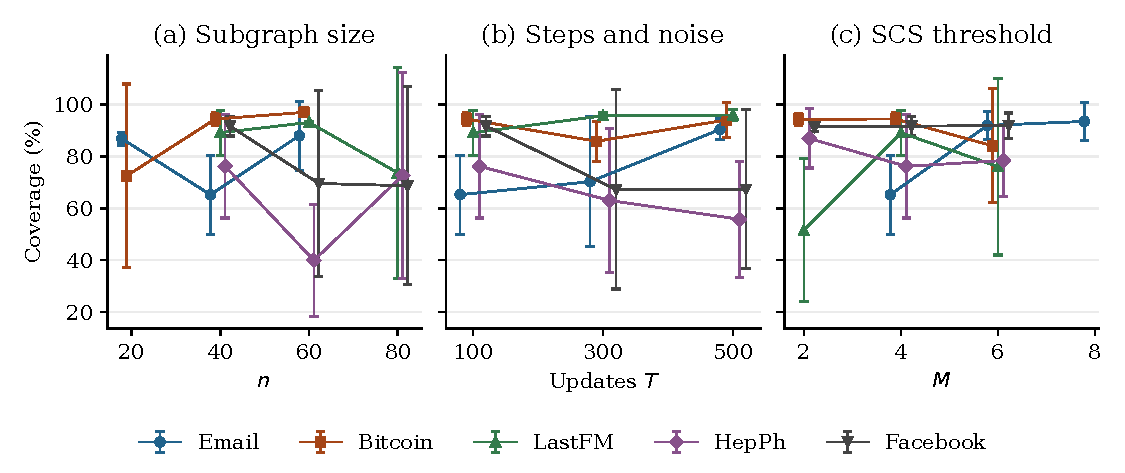
\includegraphics[width=\textwidth]{figures/parameter_sensitivity.pdf}
\caption{Exploratory PDP-PrivIM sensitivity to (a) subgraph size $n$ at $M=4$, $T=100$; (b) update count $T$ and its corresponding noise scale at $n=40$, $M=4$; and (c) SCS threshold $M$ at $n=40$, $T=100$. Points show mean Coverage and bars show one sample SD from five saved fits. Small horizontal offsets separate datasets.}\label{fig:parameter-sensitivity}
\end{figure}

Across the tested subgraph sizes, the range of mean Coverage is 19.44--36.28 percentage points across datasets. The highest tested mean occurs at $n=60$ on LastFM and $n=40$ on Facebook. From 100 to 500 updates with the corresponding noise adjustment, the mean rises from 65.201\% to 90.355\% on Email and falls from 76.144\% to 55.715\% on HepPh. The tested $M$ values produce a 37.62-point mean range on LastFM and a 0.46-point range on Facebook. These ranges describe the observed means at the tested settings. With five fits per point and substantial variation in some cells, the sweep provides exploratory evidence about sensitivity.

\subsection{Interpreting the three parameter slices}
Subgraph size $n$ changes the training examples seen by GRAT3. Larger subgraphs can include more neighborhood structure and change the terms of the coverage surrogate in Equation~\eqref{eq:loss}. The observed ranges describe how much the saved mean Coverage changes over the tested sizes. They leave open whether the differences arise from the available graph context, the resulting gradients, or their interaction with training noise.

The SCS threshold $M$ controls how frequently a node can enter the subgraph cache within a slot. The large mean range on LastFM and the smaller range on Facebook show why a threshold selected on one graph need not transfer to another. Varying $M$ alters the sampler's output while the conditional update sensitivity bound remains fixed by the two affected slots and the norm bound on each slot sum.

The update-count slice changes the number of optimization steps and the Gaussian scale per step together. At 300 and 500 steps, the multiplier on the reference scale is at least $\sqrt{3}$ and $\sqrt{5}$, respectively. The opposite directions observed on Email and HepPh concern this joint schedule. Identifying the separate effects of training duration and noise scale would require additional controlled comparisons.

\subsection{Computational work and timing evidence}
The private update consumes up to four cached subgraphs from each of four slots. A schedule of 100, 300, or 500 updates therefore reserves 1,600, 4,800, or 8,000 gradient positions, respectively. Empty positions contribute zero, so the reserved count is an upper bound on the number of evaluated subgraph gradients. The slot caches can be reused, and the cost of each gradient depends on the graph structure of its subgraph. These counts describe algorithmic work.

The saved development artifacts include separate training and final evaluation times. A wall-clock comparison would require matching hardware, the timing boundaries for cache construction and training, and the update schedules. In particular, a ratio between runs with different update counts combines computational cost per update with the chosen training duration. The available chapter evidence supports the workload comparison above. A controlled timing comparison remains open.

\section{Verified update scales and bounded signal}
The common private kernel first clips each subgraph gradient, then clips each slot sum to norm at most 3. With four slots, the combined signal $S_t$ satisfies $\|S_t\|_2\leq12$. The pre-projection update is
\begin{equation}
 \Delta\theta_t=-\frac{0.005}{16}(S_t+Z_t),\qquad
 Z_t\sim\mathcal N(0,\sigma^2I_{2340}).
\end{equation}
Therefore the signal update has norm at most 0.00375. The Gaussian increment has coordinate SD $0.005\sigma/16$ and root mean square Euclidean norm $\sqrt{2340}\,0.005\sigma/16$.

\begin{table}[htbp]
\centering\small
\caption{Verified pre-projection update scales from frozen public constants. RMS means $\sqrt{\mathbb E\|\Delta\theta_{\rm noise}\|_2^2}$; it is not a Coverage SD or a measured gradient SNR.}\label{tab:noisescale}
\begin{tabular}{lrrr}\toprule
Configuration & Coordinate noise SD & Noise L2 RMS & Signal norm bound\\\midrule
Uniform1 & 0.151875 & 7.346732 & 0.003750\\
PDP-PrivIM & 0.081250 & 3.930351 & 0.003750\\
Uniform4 & 0.043438 & 2.101226 & 0.003750\\\bottomrule
\end{tabular}
\end{table}

Table~\ref{tab:noisescale} gives the historical 100-step reference scales. For the longer private runs, the sum-noise scale is increased by at least $\sqrt{T/100}$, retaining the original conditional ideal single-model accounting upper bounds. These are parameter-budget variants, not unchanged 100-step trajectories.

These scales make noise-driven parameter trajectories a well-motivated concern: full-coordinate random increments are large relative to the bounded signal. However, the signal bound is an upper bound rather than an observed useful gradient, and parameters can have redundant functional directions. The numbers do not identify a fraction of Coverage variance, establish a function-space SNR, or describe the final distribution after adaptive gradients and projection. Multiplying by $\sqrt{100}$ would describe only an additive independent-noise reference, not the actual trained model.

\section{Historical controlled evidence for Gaussian-path sensitivity}
A separate historical G2 diagnostic held initialization, the retained graph, slot caches, and all 100 batches fixed within each of 12 pairs, while using a fresh Gaussian path. Its 24 fits cover Bitcoin, LastFM, and Facebook and are not additional observations in Table~\ref{tab:coverage}.

In one LastFM condition, Coverage changed from 96.848\% to 50.118\%, a difference of $-46.730$ pp, while Top-50 overlap was 14\%. A Facebook condition changed from 72.632\% to 93.031\%, or $+20.399$ pp. The Bitcoin changes were smaller in the saved conditions. Thus a changed Gaussian-driven training path can materially change final selection and Coverage even with the outer retained graph fixed.

This is a conditional path effect: later gradients respond to previous noisy states. It does not separate direct noise from the optimizer's response, nor establish how much of the variance in all five current graphs or either Uniform mechanism it explains. Its controls and scalar records support a specific existence result, not a universal causal ranking of instability factors.

\section{What outer sampling does and does not explain}
PDP-PrivIM's one-time Bernoulli sampling changes the retained graph and may change what useful structure is available. Initialization, retention, and Gaussian paths vary together across the five historical ordinary PDP-PrivIM repeats, so their variance contributions cannot be separated from this table.

Uniform1 and Uniform4 do not have that outer sampling, yet their saved Coverage results can be unstable. Bernoulli sampling is therefore not a necessary cause shared by all unstable configurations. The fixed-retained-graph G2 differences also show that holding retention fixed need not remove path sensitivity. This does not prove that retention has no additional effect on PDP-PrivIM.

\section{Representation, loss, projection, and final ranking}
Gaussian noise enters all 2340 coordinates, including hidden-layer and attention parameters. The post-update constraint applies only to the final 32 feature-map weights. It does not fix hidden representations, attention, or ordering of candidate nodes. Multilayer nonlinear responses are a plausible route from parameter differences to different selected sets, but existing data do not isolate a dominant layer.

The unchanged training objective is a continuous coverage surrogate plus selection penalty on sampled training subgraphs. Final evaluation instead chooses a hard Top-50 set on the held-out graph. Lower surrogate loss does not mathematically ensure higher final Coverage. Whether a particular low run suffered poor surrogate optimization, poor transfer, redundant selected neighborhoods, or several interacting effects remains unresolved without additional controlled measurements.

The ranking interface itself is discrete: changed scores can change selected identities and the union of their outgoing neighborhoods. However, small score gaps or tied scores are not a general established cause. The saved ranking audit records finite logits and zero selected zero-outdegree nodes in all 100 runs. One large boundary tie occurs in a high-utility Email Uniform1 run. Historical severe-loss examples include large boundary score gaps and no boundary ties. Those counterexamples rule out a simple common explanation based solely on sigmoid saturation or incorrect tie breaking; ranking uses pre-sigmoid scores.

\section{Measurement checks and uncertainty}
The main five-run table was checked against all 100 raw evaluations and frozen source hashes. Separately, the historical five-seed evaluations reproduce the archived historical means and SDs. For each fixed cell, Coverage is a constant multiple of Spread, so a changing normalization is not the cause of within-cell variation. Fixed-model evaluation at one-step IC probability one introduces no Monte Carlo diffusion variance.

The available code and saved diagnostics support the presence of clipping, full-coordinate noise, and post-update projection. They do not constitute exhaustive implementation verification or machine-level DP certification. No new mechanism defect is established by the observed large SD alone.

Historical gradient summaries and clipping/projection counts exist, but comparable stepwise useful-gradient directions, layerwise signal norms, and functional perturbation measurements are incomplete. This prevents a quantitative variance decomposition. Five public initialization seeds also do not separate initialization from fresh secret randomness; calling one integer a bad seed would overstate the evidence.

\section{Findings from historical comparisons}
The frozen-backbone New Matched PDP reference trains 33 coordinates and freezes 2307. In the historical five-seed comparison, it had smaller observed SDs than full-training PDP-PrivIM on all five graphs and lower mean Coverage on HepPh. The comparison changes the trainable space, clipping geometry, and secret paths simultaneously, so it cannot isolate the effect of reducing the number of trainable parameters.

Neither parameter averaging (G3) nor the row-sum variant (C3) met its prespecified development criteria. Run-to-run variability therefore remains an open issue for PDP-PrivIM.

The strongest supported explanation is that Gaussian-driven adaptive training paths can cause large Coverage changes, within a system whose bounded signal and full-coordinate noise have very different scales. The roles of graph structure, initialization, outer sampling, nonlinear representation, and discrete ranking remain incompletely separated. Reporting these limits is necessary before proposing a specific remedy.
